\documentclass[11pt]{article}
\usepackage[margin=1in]{geometry}
\usepackage{amsmath,amssymb}
\usepackage{booktabs}
\usepackage{tikz}
\usetikzlibrary{arrows.meta}
\newcommand{\relu}{\operatorname{ReLU}}
\newcommand{\gelu}{\operatorname{GELU}}
\newcommand{\sm}{\operatorname{softmax}}

\title{\textbf{Hand-constructing a \texttt{log} read-out with a GELU feed-forward layer}}
\author{}
\date{}

\begin{document}
\maketitle
\vspace{-3em}

\noindent
\textit{Goal: set the weights of a GELU feed-forward (FFN) layer \emph{by hand} so that it
computes $\log(c+\beta)$ on the count vector. No training, and the data never passes
through a $\log$ --- only through GELU.}

\section{What we want, and why}

After the attention layers, a block of the residual stream holds the in-context
\textbf{count vector} $\mathbf c=(c_1,\dots,c_V)$ (how often each token followed the
current state), with $c_i\ge 0$. The model finishes with a soft-max read-out
$\mathbf p=\sm(\boldsymbol\ell)$.

The best count-based prediction is ``proportional to the (floored) counts'':
\[
p_i=\frac{c_i+\beta_i}{\sum_j(c_j+\beta_j)},\qquad \beta_i>0\ \text{a small floor.}
\]
Since $\sm(\log\mathbf u)_i=u_i/\sum_j u_j$, the soft-max gives exactly this \emph{iff}
\begin{equation}\label{eq:goal}
\boxed{\;\ell_i=\log(c_i+\beta_i)\;}
\end{equation}
So the FFN must output $\log(c_i+\beta_i)$. We build that from GELU in four small steps.

\section{Step 1: GELU can act like a ReLU ``hinge''}

GELU is the smooth gate $\gelu(z)=z\,\Phi(z)$, where $\Phi$ is the Gaussian CDF.
A \textbf{ReLU hinge} $\relu(c-x)$ is $0$ to the left of $x$ and a line of slope $1$ to
the right. GELU becomes the same hinge if we feed it a large \textbf{gain} $g$ and divide by $g$:
\begin{equation}\label{eq:gain}
\frac{\gelu\!\big(g\,u\big)}{g}=u\,\Phi(g\,u)\;\xrightarrow[g\to\infty]{}\;u\,\mathbf 1[u>0]=\relu(u).
\end{equation}
For finite $g$ the corner is just rounded over a width $\sim 1/g$ (Fig.~\ref{fig:hinge}).
So a large input weight $g$ turns GELU into a sharp hinge.

\begin{figure}[h]
\centering
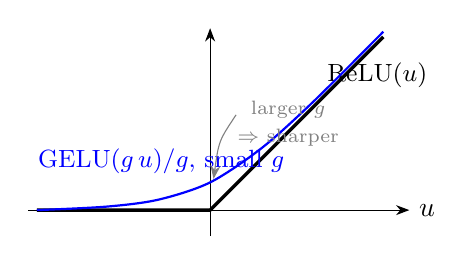
\begin{tikzpicture}[scale=2.2]
  \draw[-{Stealth}] (-1.05,0) -- (1.15,0) node[right]{$u$};
  \draw[-{Stealth}] (0,-0.15) -- (0,1.05);
  % ReLU: two straight segments, sharp corner at 0
  \draw[very thick] (-1,0) -- (0,0) -- (1,1);
  \node[right] at (0.62,0.78) {\small $\relu(u)$};
  % GELU small gain (rounded)
  \draw[blue,thick] plot[smooth] coordinates{(-1,0.0)(-0.6,0.02)(-0.3,0.06)(0,0.16)(0.3,0.36)(0.6,0.63)(1,1.03)};
  \node[blue,right] at (-1.05,0.28) {\small $\gelu(g\,u)/g$, small $g$};
  % arrow indicating sharpening
  \draw[-{Stealth},gray] (0.15,0.55) .. controls (0.05,0.4) .. (0.02,0.18);
  \node[gray,align=center] at (0.45,0.5) {\scriptsize larger $g$\\[-2pt]\scriptsize $\Rightarrow$ sharper};
\end{tikzpicture}
\caption{The gain trick: $\gelu(g\,u)/g\to\relu(u)$ as the gain $g$ grows.}
\label{fig:hinge}
\end{figure}

\section{Step 2: A sum of hinges is a piecewise-linear curve}

Pick break-points (\emph{knots}) $0=x_0<x_1<\dots<x_{K-1}$. A hinge $\relu(c-x_k)$
``switches on'' an extra $+1$ of slope at $x_k$. To make a curve whose slope is $m_k$ on
the piece $[x_k,x_{k+1}]$, add a hinge at each knot with weight equal to the
\textbf{slope change} there:
\begin{equation}\label{eq:pl}
\hat h(c)=\underbrace{\log\beta}_{\text{value at }c=0}
+\,m_0\,\relu(c-x_0)
+\sum_{k\ge 1}\big(m_k-m_{k-1}\big)\,\relu(c-x_k).
\end{equation}
Check: for $c$ in piece $k$, the active hinges are $x_0,\dots,x_k$, and their slopes add up to
$m_0+\sum_{j=1}^{k}(m_j-m_{j-1})=m_k$ --- the right slope on every piece, and the curve is continuous.

\section{Step 3: Choose the slopes to trace $\log(c+\beta)$}

Set each $m_k$ to the straight-line (secant) slope of $\log(c+\beta)$ across that knot interval:
\begin{equation}\label{eq:slopes}
m_k=\frac{\log(x_{k+1}+\beta)-\log(x_k+\beta)}{x_{k+1}-x_k}.
\end{equation}
Then $\hat h$ is the piecewise-linear interpolant of $\log(c+\beta)$ (Fig.~\ref{fig:log}).
Because $\log$ is \textbf{concave}, the slopes $m_k$ \emph{decrease}, so the first hinge
weight $m_0$ is positive and every later weight $(m_k-m_{k-1})$ is negative --- the hinges
bend the line downward, exactly like $\log$ flattening. More knots $\Rightarrow$ smaller error.

\begin{figure}[h]
\centering
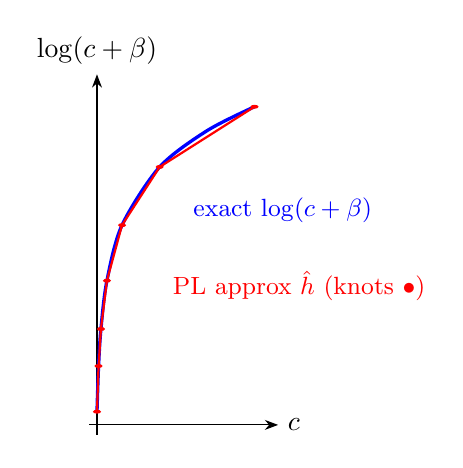
\begin{tikzpicture}[scale=2.0,yscale=0.42]
  \draw[-{Stealth}] (-0.05,-4.8) -- (1.15,-4.8) node[right]{$c$};
  \draw[-{Stealth}] (0,-4.95) -- (0,0.5) node[above]{$\log(c+\beta)$};
  % smooth log curve  (beta=0.01)
  \draw[blue,very thick] plot[smooth] coordinates{
    (0,-4.6)(0.01,-3.91)(0.025,-3.35)(0.063,-2.62)(0.159,-1.78)(0.398,-0.90)(0.7,-0.35)(1.0,0.01)};
  % piecewise-linear approx through the knots
  \draw[red,thick] (0,-4.6)--(0.01,-3.91)--(0.025,-3.35)--(0.063,-2.62)--(0.159,-1.78)--(0.398,-0.90)--(1.0,0.01);
  \foreach \x/\y in {0/-4.6,0.01/-3.91,0.025/-3.35,0.063/-2.62,0.159/-1.78,0.398/-0.90,1.0/0.01}
     \filldraw[red] (\x,\y) circle (0.6pt);
  \node[blue,right] at (0.55,-1.55) {\small exact $\log(c+\beta)$};
  \node[red,right]  at (0.42,-2.7) {\small PL approx $\hat h$ (knots $\bullet$)};
\end{tikzpicture}
\caption{The hinge sum \eqref{eq:pl} is the piecewise-linear interpolant of $\log(c+\beta)$
($\beta=0.01$); knots clustered near $0$ where $\log$ is steep.}
\label{fig:log}
\end{figure}

\section{Step 4: Write it into GELU-FFN weights}

The residual FFN is $\mathrm{FF}(\mathbf s)=\mathbf s+W_2\,\gelu(W_1\mathbf s+\mathbf b_1)$,
and the read-out is $\boldsymbol\ell=W_o\mathbf s+\mathbf b_o$. Use one hidden unit per
(coordinate $i$, knot $k$). Combining the gain trick \eqref{eq:gain} with the hinge sum
\eqref{eq:pl}: a hinge $\alpha_k\,\relu(c_i-x_k)$ is realized as
$\dfrac{\alpha_k}{g}\,\gelu\!\big(g(c_i-x_k)\big)$. So set
\[
\boxed{\;
W_1[u,\,\text{index of }c_i]=g,\quad
b_1[u]=-g\,x_k,\quad
W_2[\text{out }i,\,u]=\frac{\alpha_k}{g},\quad
b_o[i]=\log\beta_i,\;}
\]
where $\alpha_0=m_0$ and $\alpha_k=m_k-m_{k-1}$ for $k\ge1$. Then the unit computes
$\gelu\!\big(g(c_i-x_k)\big)$, the output coordinate accumulates
$\sum_k \tfrac{\alpha_k}{g}\gelu(g(c_i-x_k))\approx\hat h(c_i)-\log\beta_i$, and adding
$b_o[i]$ gives $\ell_i\approx\log(c_i+\beta_i)$.

\paragraph{What touches the data.} Only GELU. The $\log$ in \eqref{eq:slopes} is used
\emph{once}, to compute the fixed numbers $m_k$ (the weights); the data $c$ flows solely
through $W_1,\ \gelu,\ W_2$.

\section{Concrete numbers ($\beta=0.01,\ K=7$ knots $\Rightarrow$ $6$ GELU units per coordinate, gain $g=200$)}
\[
x_k:\ 0,\ 0.010,\ 0.025,\ 0.063,\ 0.159,\ 0.398,\ 1.0;
\qquad
m_k:\ 69.3,\ 37.2,\ 19.3,\ 8.75,\ 3.69,\ 1.51 .
\]
\begin{center}
\begin{tabular}{ccccc}
\toprule
unit $u$ & $W_1$ weight & $b_1=-g\,x_k$ & $W_2$ weight $=\alpha_k/g$ & ($\alpha_k$) \\
\midrule
$0$ & $200$ & $0.00$    & $+0.3466$ & ($+69.32$)\\
$1$ & $200$ & $-2.00$   & $-0.1604$ & ($-32.08$)\\
$2$ & $200$ & $-5.02$   & $-0.0897$ & ($-17.94$)\\
$3$ & $200$ & $-12.62$  & $-0.0527$ & ($-10.55$)\\
$4$ & $200$ & $-31.70$  & $-0.0253$ & ($-5.06$)\\
$5$ & $200$ & $-79.62$  & $-0.0109$ & ($-2.19$)\\
\bottomrule
\end{tabular}
\end{center}
Read-out bias $b_o=\log(0.01)=-4.605$. With $V=20$ coordinates this uses
$20\times6=120$ of the $128$ hidden units.

\section{Does it work? (gain convergence)}
Cross-entropy of the hand GELU read-out vs.\ the idealized exact-$\log$ read-out, on test data:
\begin{center}
\begin{tabular}{cccccc}
\toprule
$\alpha$ & exact $\log$ & $g=20$ & $g=50$ & $g=200$ & $g=1000$\\
\midrule
$0.5$ & $2.2901$ & $2.2913$ & $2.2907$ & $2.2893$ & $2.2891$\\
$0.8$ & $1.5873$ & $1.6008$ & $1.5995$ & $1.5955$ & $1.5950$\\
$0.9$ & $1.2386$ & $1.2546$ & $1.2453$ & $1.2382$ & $1.2365$\\
\bottomrule
\end{tabular}
\end{center}
By $g\approx200$ the GELU construction is indistinguishable from exact $\log$, and it keeps
improving as $g$ grows (Eq.~\eqref{eq:gain}).

\section{Result}
\[
\sm(\boldsymbol\ell)_i=\frac{e^{\log(c_i+\beta_i)}}{\sum_j e^{\log(c_j+\beta_j)}}
=\frac{c_i+\beta_i}{\sum_j(c_j+\beta_j)} .
\]
A pure-GELU feed-forward layer, with hand-set weights, reproduces the divide-by-sum
(count) predictor: the $\log$ inverts the soft-max exponential. This is the same
function the trained model arrives at --- its logits regress onto $\log(\text{count})$
with slope $\approx1$ and $R^2\approx0.9$.
\end{document}
